\section{Data Collection and Segmentation}
\label{sec:method}
%Please keep in mind the following information: We are unsure if dogs have phones, words, or sentences similar to those found in the human language. As a result, we will not be directly applying the definitions of phones, words, or sentences from human language to dogs. We will provide the definitions of phones, words, and sentences based on our research on dogs at a later time. The reason for using these terms from human language is that if dogs had language, we would expect to find similar components in their language.

In this section, we detail our workflow\footnote{The code and dataset is available at \url{https://anonymous.4open.science/r/Dog_Language-67B2/}}~(\figref{fig:Workflow}) including audio clean-up by AudioSep, sentence extracting, dataset, phone recognition, word discovery, and semantics discovery. 
The first three parts are primarily intended to gather large amounts of high-quality data on dog barking, while the last three parts aim to investigate potential phones and words in dog vocalizations.
% Implementation details can be found in Appendix~\ref{sec:appendix_a}.

\begin{figure}[th]
    \centering
    \scalebox{0.35}{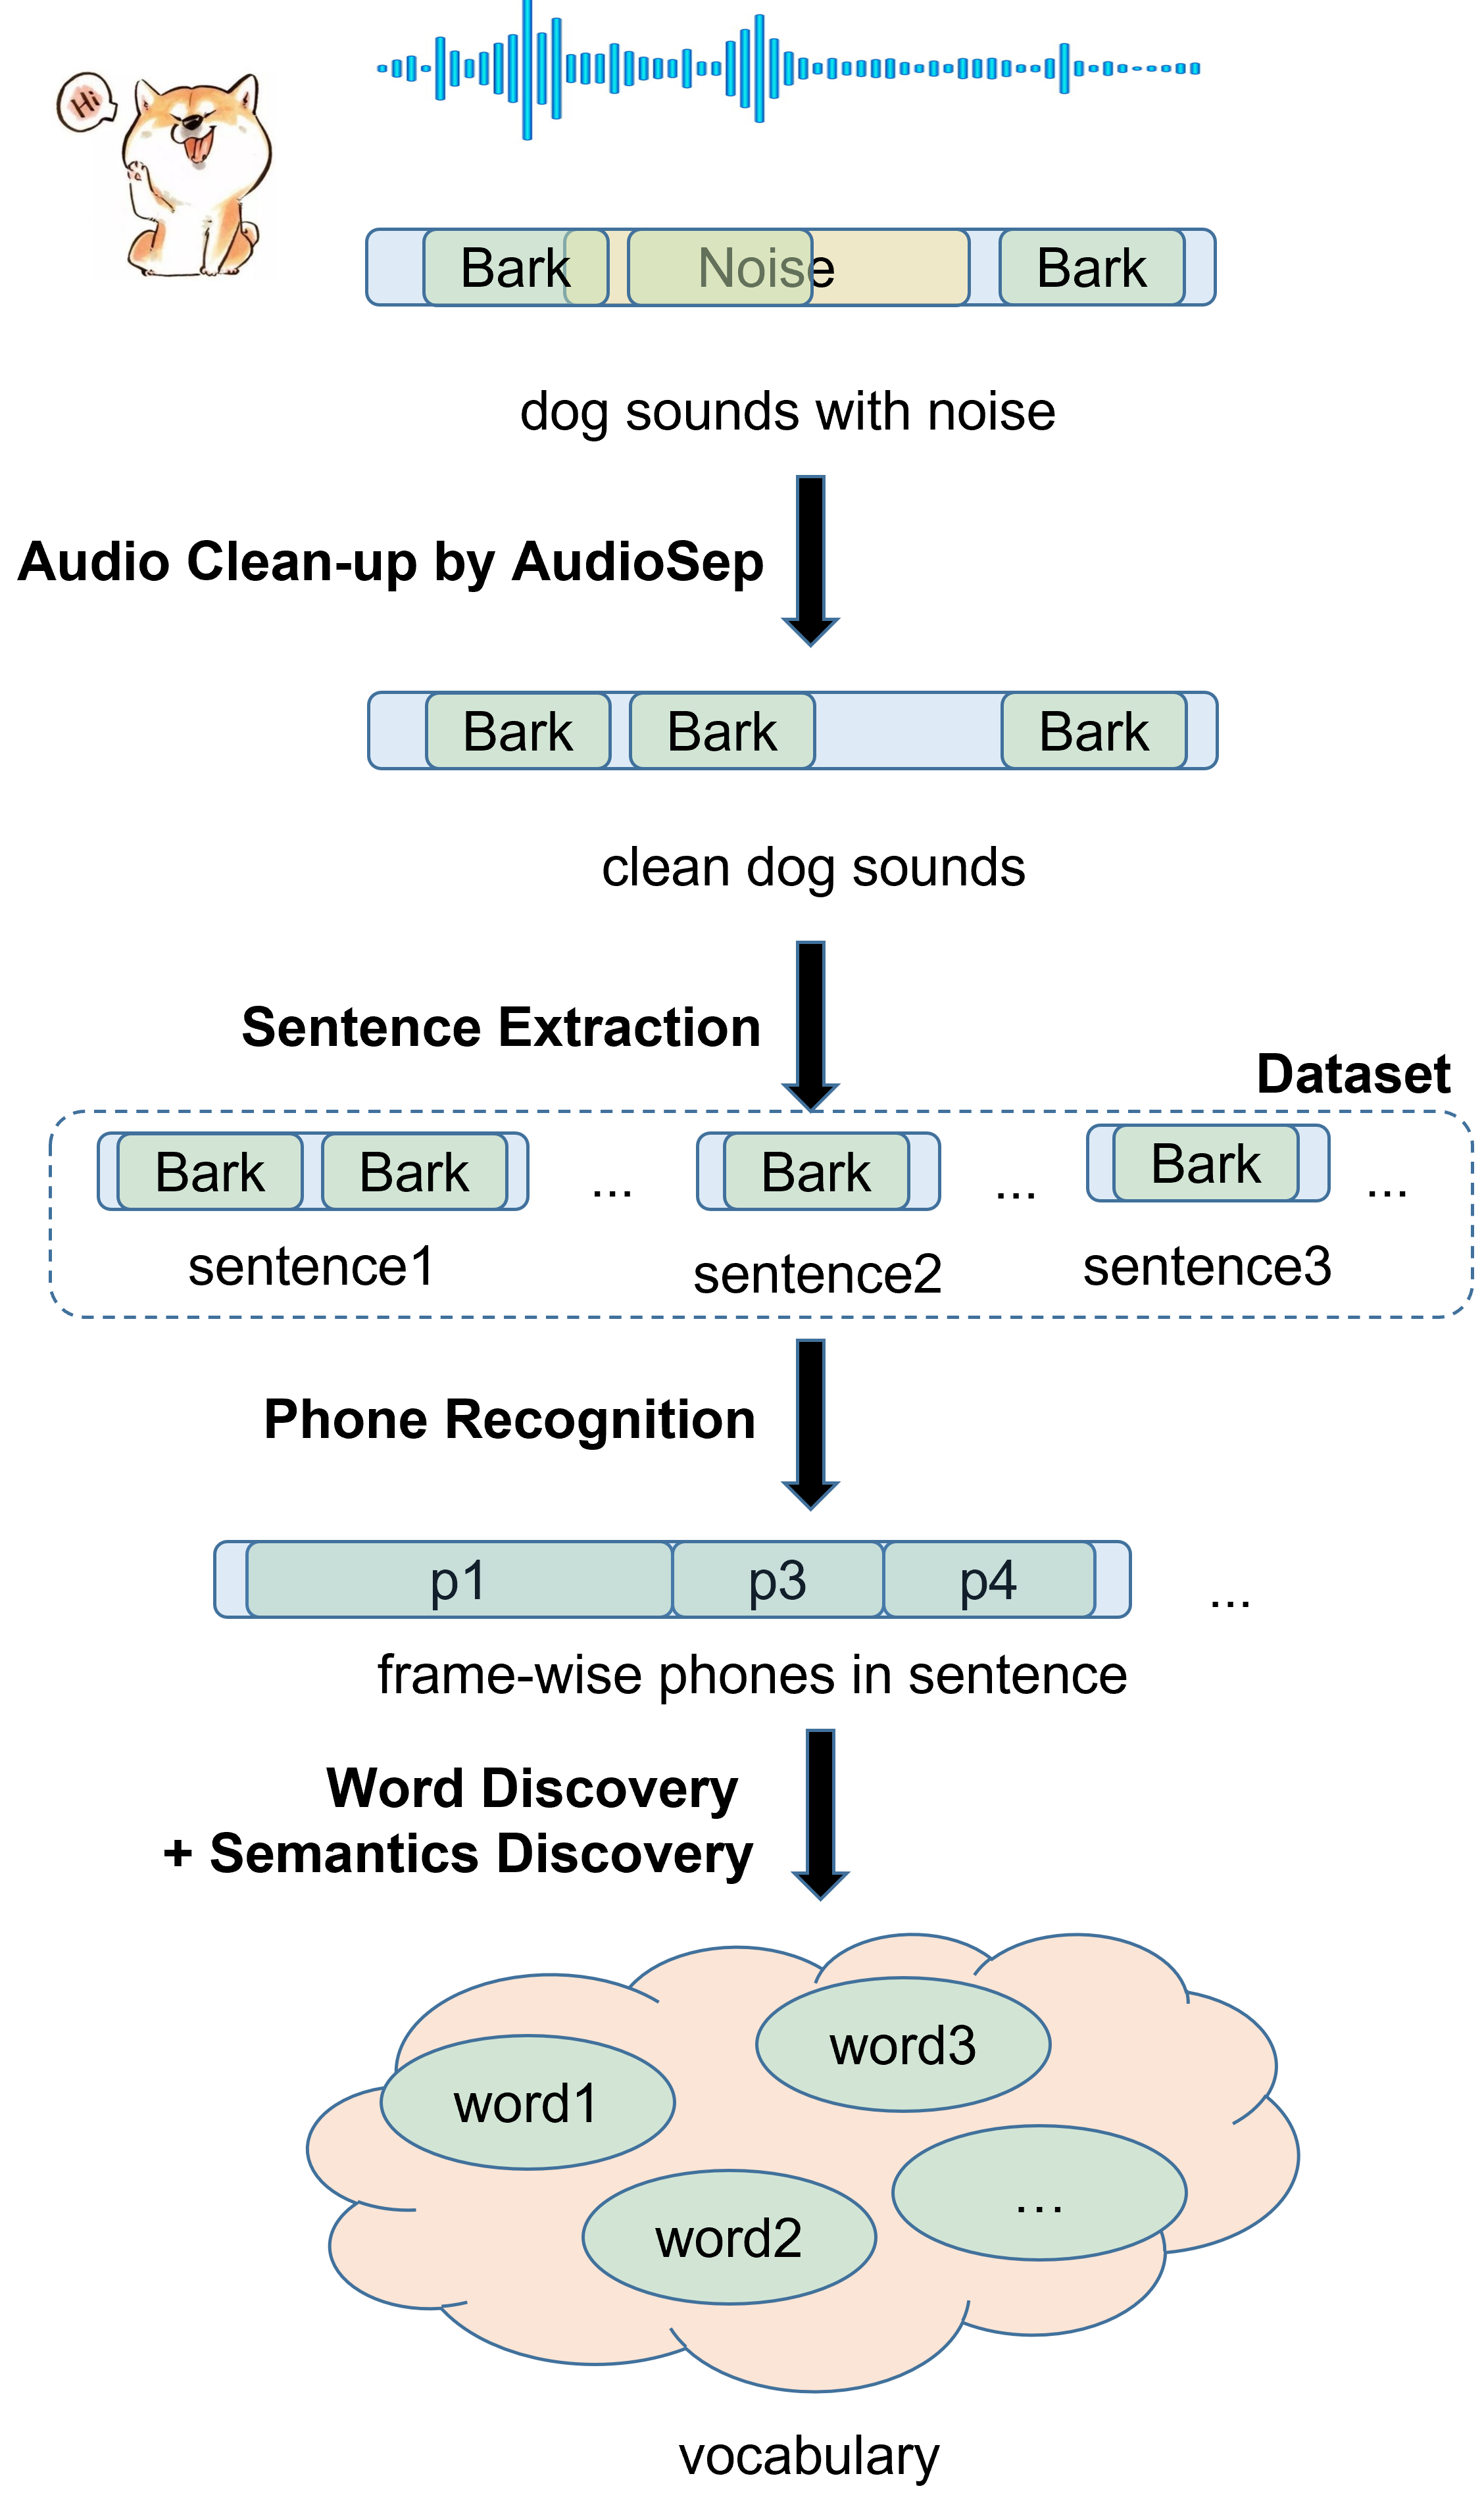
\includegraphics{workflow.png}}
%    \caption{Full pipeline from data processing to word discovery.
	\caption{A workflow to discovery phones and words in canine vocals. 
%		\KZ{``Phone recongition''
%	is not done on a single sentence but many. Combine ``phone combination''
%	into ``phone recognition''. ``Word discovery'' also done on many sentences, once a vacab is
%	obtained, use it to parse individual sentences.}
}
    \label{fig:Workflow}
\end{figure}



\subsection{Audio Clean-up by AudioSep}

A mixture of dog sounds and noises will inevitably occur due to the use of videos from 
public social media. These noises can be background music edited in by the video uploader, 
human speeches, toy noises, etc. 
We expect a cleaner dataset, so we need to separate dog sounds from all mixed audios. 
In this work, we use AudioSep~\citep{liu2023separate}, a foundation model for open-domain audio source separation with natural language queries. The AudioSep is pre-trained on large-scale multimodal datasets, including AudioSet~\citep{gemmeke2017audio} dataset, VGGSound~\citep{chen2020vggsound} dataset, AudioCaps~\citep{kim2019audiocaps} dataset, etc. 
We apply AudioSep, using ``Dog'' as the input text query, to separate dog sounds from all audio. 
After this step, we will be working with higher quality dog vocals. 


\subsection{Sentence Extraction}
After the separation of dog sounds, the audio will contain mostly barking, silence, and 
a small amount of noise that can not be removed. 
Next we segment the dog vocalization audio clips into ``sentences'' to contain the length
of a single vocal sequence.
%To focus on the part of dog sounds, we need to eliminate as much interference as possible from remaining silences and noises. 
using a approach similar to \citet{huang2023transcribing}, 
which defines a sentence as \textit{a continuous sequences of dogs barks with no more than 
0.5 seconds silence in between}.
We apply PANNs~\cite{kong2020panns} trained on the large-scale AudioSet dataset to 
extract clips of dog sounds. In order to acquire higher quality data, we initially manually 
labeled some dog barking data from our dataset. 
The data consisted of 1,483 dog barking audio clips with a total duration of more 
than 9,597 seconds. We utilized this data to fine-tune the pre-trained PANNs model 
and achieved an F1 score of 0.8111. Then, consecutive clips less than 0.5 second apart 
are combined to form a dog ``sentence''. 

To further reduce noise, sentences that meet one of the following conditions will be removed: 
(1) ``Dog'' label score less than 0.1; 
(2) One of the top 10 sound event tags is not related to dogs and has a score greater 
than the score for the dog tag, or the 
difference between the score and the score for the dog tag is less than 0.7. 
With this process, we obtain more and cleaner sentences 
than \citet{huang2023transcribing}.

To verify the effectiveness of AudioSep and to confirm that it did not have a significant impact on sound quality, we manually labeled 1,467 seconds~(1,137 seconds for train and 330 seconds for test) audios of dog barking to fine-tune PANNs. The result~(\tabref{tab:audioSepRes}) shows that AudioSep can effectively reduce noise interference without significantly impacting the quality of dog sounds. The setting with the highest $F1$ score is adopted for all following experiments and analysis.
%\MY{The setting with the highest $F1$ score is adopted for all following experiments and analysis.}

\begin{table}[th]
	\centering
 	\small
	\begin{tabular}{lcc}
		\hline
		\textbf{Train Data} & \textbf{Test Data} & \textbf{F1 Score}\\
		\hline
		~~~~~~~~~- & - & 0.6916 \\
		\hline
		~~~~~~~~~\Checkmark{} & - & 0.6797 \\
		\hline
		~~~~~~~~~- & \Checkmark{} & \pmb{0.7755} \\
		\hline
		~~~~~~~~~\Checkmark{} & \Checkmark{} & 0.7709 \\
		\hline
	\end{tabular}
	\caption{The result of PANNs. Those with a check mark are using AudioSep.}
	\label{tab:audioSepRes}
\end{table}

\subsection{Dataset}

Our raw dataset contains more than 6.8k YouTube videos of various types of dogs, including
those from \citet{huang2023transcribing} and AudioSet~\citep{gemmeke2017audio}. 
After the sentence extracting in our workflow contains 37,919 dog ``sentences''~(more than 23 hours) from more than 1,300 users. Compared to previous studies~\citep{huang2023transcribing, abzaliev2024towards, Yin2004BarkingID}, our dataset significantly exceeds them in terms of dog barking duration and number of dogs.

Obviously, mispronunciation problems can arise in human speech datasets due to various reasons, such as differences in phonetics for non-native speakers, speech disorders, or simply errors in articulation. This might also be the case with our dog dataset or other dog  dataset~\citep{huang2023transcribing, abzaliev2024towards, Yin2004BarkingID}. But with a large amount of data, it can still achieve good results~\citep{huang2023transcribing, abzaliev2024towards, hagiwara2023aves}. We possess the largest amount of high-quality dog datasets compared to these previous studies. We think that our extensive collection of high-quality datasets can help mitigate the impact of mispronunciation problems. Furthermore, it is simple to expand our dataset.
\section{Phonetic and Lexical Discovery}
In this section, we detail our approach in training a model to identify canine phones from the above segmented data and discover possible semantic units.
\subsection{Phone Recognition}

%Some scholars~\cite{ladefoged2006course} consider a phone to be the smallest unit of sound in a language that can distinguish one word from another.  If dogs have language, we assume that they also have minimal units. These minimal units in dog barks may be nothing like the phones in human language.

%Dog barks is unfamiliar territory for humans. The lexicon, length, and other information of dog sound units are unknown, making it can not easily delineate sound units in a dog sentence in the same way that we delineate words in a human sentence. So directly using a priori knowledge of human language or the way to split human language units like \citet{huang2023transcribing} to understand dog sound may be inapplicable. %In order to find out the minimal units in dog vocalizations, we utilize a self-supervised approach 
%Self-supervised approaches for speech representation learning can be a more appropriate method for discovering the sound units of dog language. 
After extracting clean dog vocaliztions, we endeavor to discover minimal sound units (referred as phones) from these clips. 
%In this work, we use HuBERT~\citep{hsu2021hubert}, a self-supervised approach that learns a combined acoustic and language model over continuous inputs, to understand dog sound units.  ~\citeposs{hsu2021hubert} work has demonstrated the good ability of HuBERT in characterizing human language. Interestingly, \citet{hsu2021hubert} supposed that the classes of Hubert outputs can be thought of as phone~(sub-phone) in human languages, or as units that contain phonetic information.
In our study, we have meticulously isolated distinct vocalizations from dogs, aiming to identify the fundamental sound components, which we refer to as phones, within these recordings. To achieve this, we have employed HuBERT~\citep{hsu2021hubert}, a self-supervised learning technique that assimilates acoustic and linguistic data from ongoing audio streams. Since there is no established phone set for canine vocalizations, it is difficult to manually label each audio clip with designated phone labels. Such a self-supervised method has been instrumental in our analysis of canine vocalizations. The research by ~\citeposs{hsu2021hubert} has already established HuBERT's proficiency in delineating the nuances of human speech, where they have posited that the output classes from HuBERT could be analogous to phones (or sub-phones) in the context of human languages, serving as carriers of phonetic information.


%A number of researchers~\citep{hagiwara2023aves, abzaliev2024towards} have shown that self-supervised methods are equally adept at analyzing and characterizing the vocalizations of animals. Specifically, the work by ~\citeposs{hagiwara2024ispa} has utilized HuBERT to establish a phonetic alphabet that transcends species, facilitating the transcription of animal sounds.

Specifically, we pretrain a Dog-HuBERT using all sequences of dog vocalizations, which is a total of more than 20 hours' data.
%\MY{which is a total of xx hours' data. }. 
We used 100 clusters at the first stage and 150 clusters at the second stage, a learning rate of 0.0001, and 80k training steps at the first stage and 60k training steps at the second stage. Then we used features, which are from the 11th transformer layer of the second-stage model, to train a K-Means model with 140 clusters. \figref{fig:cluster} illustrates the clusters respectively indicating dog phones and noise labels. The clusters are determined based on the sum of distances from each sample to its cluster center for different clusters~(\figref{fig:clusters}). It is a good choice when the curve flattens out, allowing for enough clusters without adding too many noise labels. Clearly, the cluster centers are evenly distributed, and the noise phones are mainly concentrated in one corner of the image, indirectly indicating the reliability of the phone discovery results.
%\MY{the cluster number is determined by the sum? unclear sentence. this para needs more details}

\begin{figure}[th]
	\scalebox{0.5}{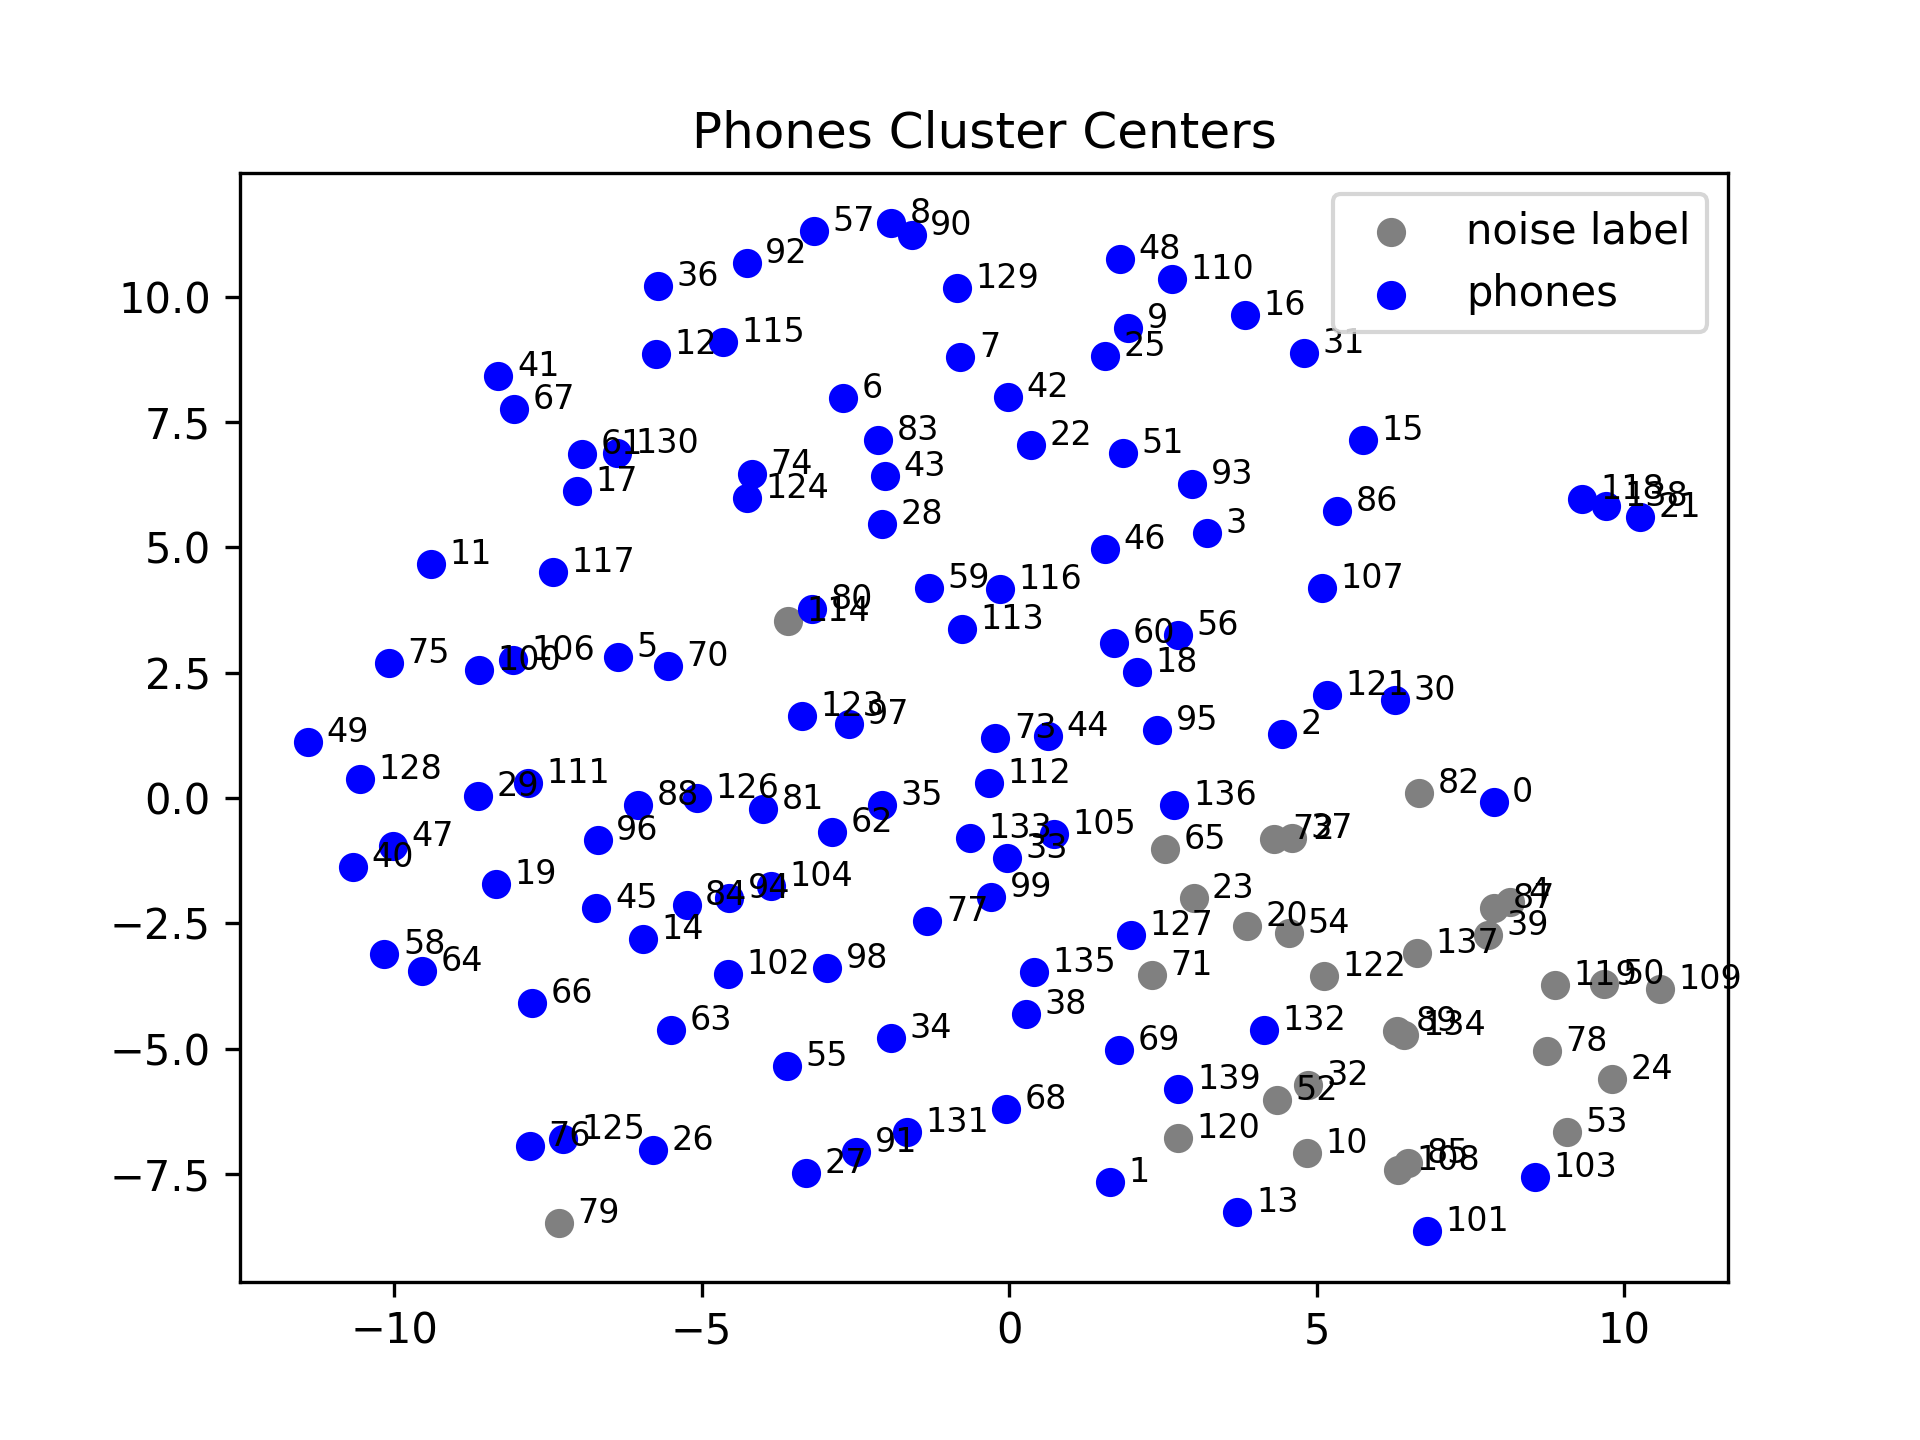
\includegraphics{phoneclustercenter.png}}
	\caption{t-SNE plot of 140 different phones from Dog-HuBERT.}
%		\KZ{Change phoneme to phone in pic.}
	\label{fig:cluster}
\end{figure}

\begin{figure}[h]
	\centering
	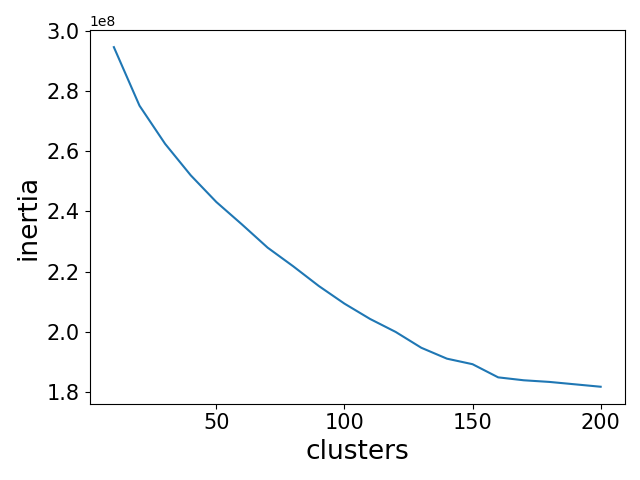
\includegraphics[width=0.95\columnwidth]{clusters.png}
	\caption{Inertia under different clusters. 140 is a suitable clusters. 
		This is the basis for our choice of 140 clusters in the third K-Means model, which is trained based on the HuBERT of second stage. 
%		\MY{what is the third model?} 
		The same method was used for the others.}
	\label{fig:clusters}
\end{figure}

We regard the distinct classes produced by Dog-HuBERT as the basic units of canine vocal expression. Consequently, we define these output classes as the fundamental components within a dog's bark, dubbing them as the dog's ``phone''. This terminology aligns with the concept of phones in linguistics, signifying the smallest units of sound that carry meaning.

%Several scholars~\citep{hagiwara2023aves, abzaliev2024towards} have demonstrated that self-supervised approach are equally strong at characterizing animal sounds. \citeposs{hagiwara2024ispa} work used HuBERT to found the inter-species phonetic alphabet for transcribing animal sounds. So we use dog ``sentences'' to pre-train HuBERT. We consider the HuBERT output classes to be the unit for dog barking. Thus, we define the classes of HuBERT outputs as the sufficiently small units in the dog's barks, and we call it as dog ``phone''.

%\subsection{Phoneme Combination}
%\XY{TODO: sinong's work}
%After K-means clustering the features extracted from the approximately 20ms audio frames using HuBERT, we obtained a transcript with labels for each dog sound sentence. However, interestingly, the duration of a phone is often longer than 20ms. With the help of the excellent context recognition ability of the Transformer-based model, a large number of labels appear continuously in the transcript. After observing it, we found that there are still some noise segments in the transcript, such as a transcript containing the sequence: $[27, 27, 27, 5, 27, 27]$. After manual review of the original video, we found that the segment contains some faint noise. In order to obtain a purer transcript, we designed a phone combination algorithm.
% \MY{Training details should be reported for the two-step hubert pretraining, on what GPU, for how many epochs, optimizer, learning rate etc.}



% \begin{algorithm}
% \caption{An algorithm with caption}\label{alg:cap}
% \begin{algorithmic}
% \Require $n \geq 0$
% \Ensure $y = x^n$
% \State $y \gets 1$
% \State $X \gets x$
% \State $N \gets n$
% \For{\texttt{i in abc}}
% \EndFor
% \While{$N \neq 0$}
% \If{$N$ is even}
%     \State $X \gets X \times X$
%     \State $N \gets \frac{N}{2}$  \Comment{This is a comment}
% \ElsIf{$N$ is odd}
%     \State $y \gets y \times X$
%     \State $N \gets N - 1$
% \EndIf
% \EndWhile
% \end{algorithmic}
% \end{algorithm}

%The algorithm uses double pointers to probe whether there are segments with the same label on both sides of the label. tolerance refers to the maximum length that can be assimilated by the labels on both sides. For example, when $tolerance=1$, the transcript segment $[a, a, b, b, a, a]$ cannot be optimized to $[a, a, a, a, a, a]$. After global phone combination optimization, we obtain the mean and standard deviation of the length of each phone.

\subsection{Word Discovery}
%\XY{TODO: sinong's work}
%\XY{give the definition of our dog word}
%\XY{\citep{trask2013dictionary} say the definition of human word: A word is a minimal free form, that is, the smallest unit of language that can stand on its own and convey meaning.}
%\XY{\citep{matthews2014concise} say the definition of human word: The smallest unit of language that can stand alone as a complete utterance, having meaning, and consisting of one or more morphemes, which are arranged in a complex yet constrained order.}

%We define ``words'' in canine language similarly to the definition of human ``words'',
%which are the smallest units of language that can stand on their own and convey meaning~\citep{trask2013dictionary,matthews2014concise}{}.
We define a ``word'' as the smallest sequence of phones that consistently appears in 
one or more specific situations.
In our proposed pipeline,
after phone recognition step,
we acquire a set of phones and can transcribe each sentence into a phone sequence.
We continue to explore the potential words from these sentences.

The lack of prior knowledge in animal language prevents us from using discriminative deep learning method~\citep{baevski2021unsupervised},
while brute-force methods fail to capture the language structure.
Adaptor Grammar~\citep{johnson2006adaptor} can statistically learn recurrent sequence segment,
and build context-free grammar (see Appendix \ref{sec:pcfg} for more discussion about
Probabilistic Context-Free Grammars (PCFGs). We use Hybird Variational-MCMC Inference~\citep{zhai2014online} to train the 
parameters of the Adaptor Grammar, ultimately obtaining a candidate vocabulary.
%\MY{We don't know whether this is accurate or not, instead you can say After phone recognition step, we acquire a set of phones and can transcribe each sentence into phone sequences. We would like to discover possible words from these sequences. There are different ways of identifying words from phone sequences: xxxxx and we use xxx since xxxx} 


We use $\mathbf{S}_{i}=\{p_{j}|1 \leq j \leq J_{i}\}$ to denote a sentence, or a
series of phones, where a phone $p_{j} \in \mathbb{P}$, in which $\mathbb{P}$ 
is a set of integers, and $J_{i}$ stands for the length of sentence $i$.

To discover the latent hierarchical linguistic structures in canine sentences, we use underlines to indicate adapted non-terminals and use ${}^{+}$ to indicate right-branching recursive 
rules for non-terminals.

$$\text{Sentence} \rightarrow \underline{\text{Word}}^{+} $$
$$\underline{\text{Word}} \rightarrow \text{Phone}^{+}$$
$$\text{Phone} \rightarrow p \; \; \text{for} \; p \in \mathbb{P} $$

We treat the nonterminal \textit{Word} as an adapted nonterminal,
learning the relationship between \textit{Word} and observation segments during training.
We parse the entire training data using the trained model as \figref{fig:parse},
obtaining the parse results for each utterance.
By calculating the occurrence counts of each word across all sentences, 
we ultimately obtained a ranked list of candidate words. 

\begin{figure}[th]
    \centering
    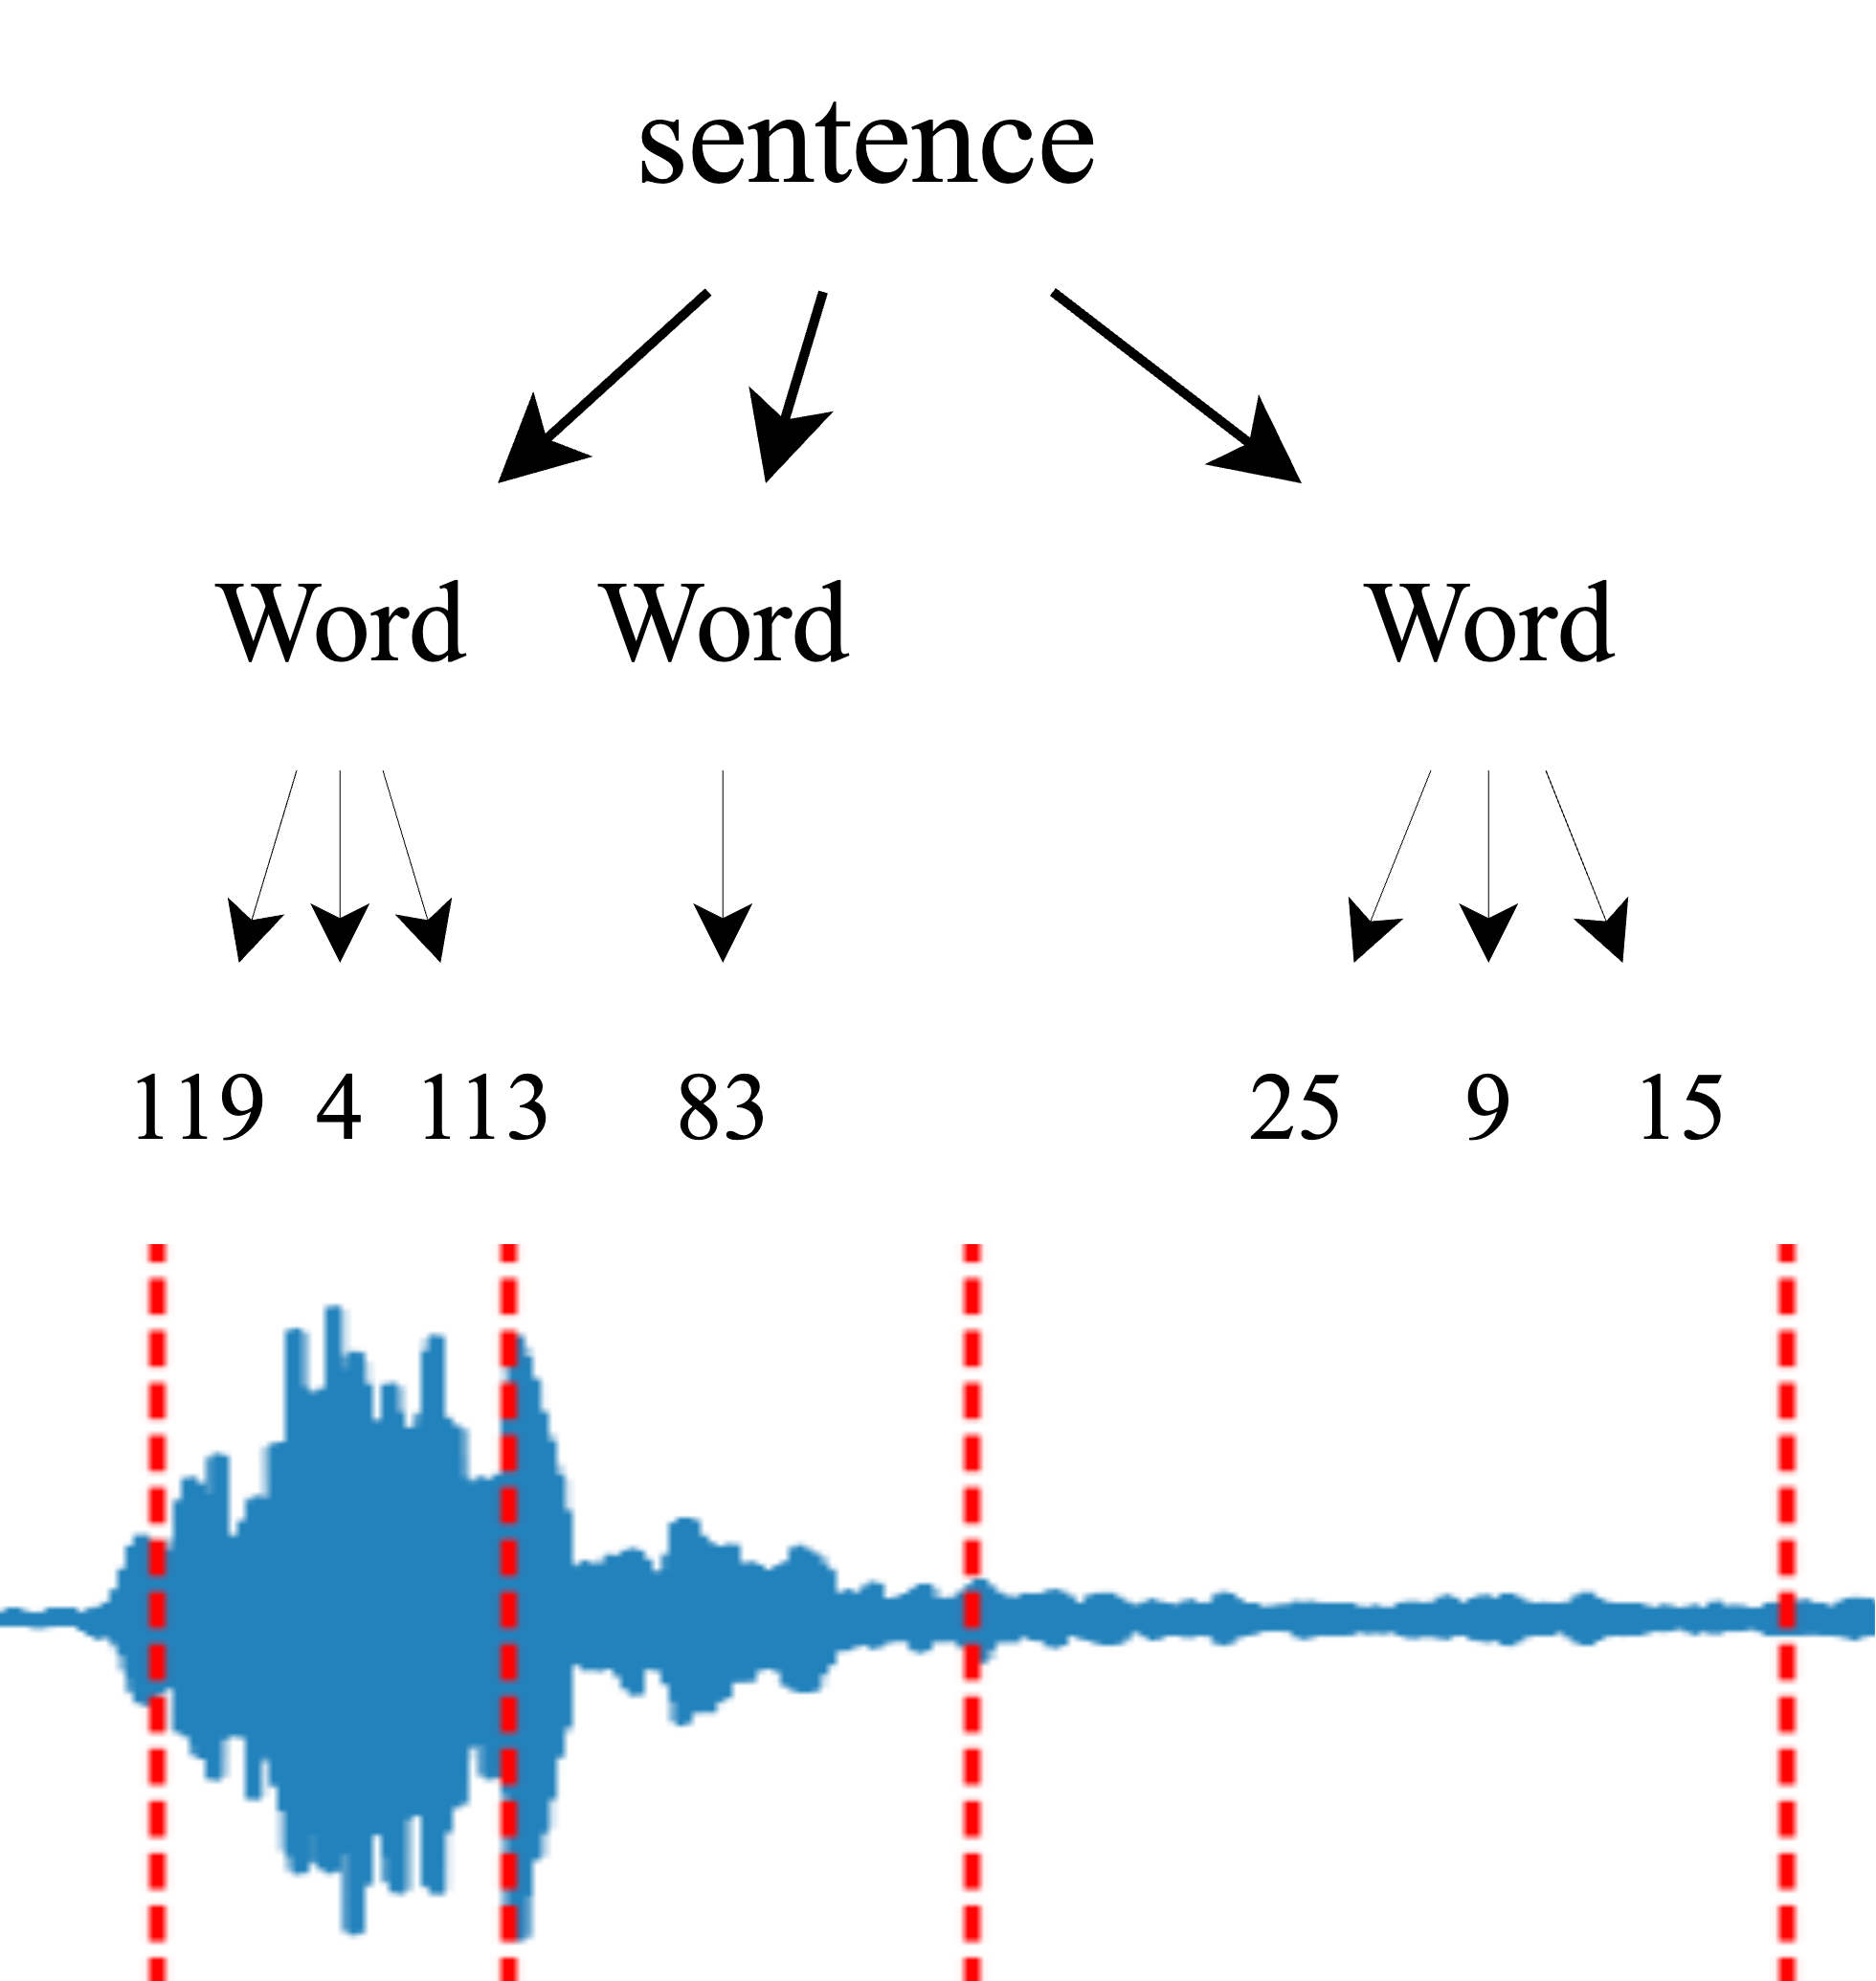
\includegraphics[width=0.6\columnwidth]{parse.png}
    \caption{Parsing a sentence.}
    \label{fig:parse}
\end{figure}

\subsection{Semantics Discovery}
To thoroughly understand dog vocalization, we need to obtain complete contextual information
such as weather, environment, and the vocalization target,
since these factors could be reactions to or causes of changes in the context.
It is very challenging to obtain complete contextual information.
But we can obtain partial context to explore coarse-grained semantics behind that dog barking sound~\citep{berthet2023animal}.

%Here for each dog sentence, we take out the video segment that spans 5 seconds before and  after the sentence.   We apply a dog activity annotation method in \citet{wang2023towards} to annotate each video segment with some of the 16 dog activities  (See \tabref{tab:acts}). This method
%three contexts: before, during, and after the dog barked. For each extracted dog ``sentence'', we extended it for 5 seconds before and after and then a video understanding model is applied to decide what the dog is doing. We defined the categories of activities~(\tabref{tab:behaviorCategories}) based on \citeposs{wang2023towards} work. 
%uses the Temporal Segment Networks~(TSN)~\citep{wang2016temporal} to detect the dog's  activities in the videos. This activity detection algorithm has a 0.61 top-1 accuracy and 0.92 top-5 accuracy. Then each activity can be classified into one of the three relative positions to every word in the sentence as ``before'', ``during'' or ``after'' using the position classification algorithm~(Algorithm~\ref{alg:pca}).

We believe the meaning of a word is determined by a causal relation between the context
and the word. Specifically, if a contextual event causes a word to be uttered, this usually
means that this word is a \textbf{reaction} to the event. On the other hand, if a word causes an
event to occur, this means that the word is a \textbf{request} to the event.
We boardly categorize the dog events into 14 different dog activities, 
after \citet{wang2023towards}. 
We implemented a method for recognizing canine activities in three distinct phases: 
before, during, and after the utterance of a word. 
For each isolated segment of a dog's vocalization, which we refer to as a ``sentence'', 
we expanded the analysis to include a 5-second window both before and after the vocalization. To ascertain the dog's activities within these time frames, we employed a video understanding model, called Temporal Segment Network (TSN)~\citep{wang2016temporal}, 
one of the state-of-the-art models designed for video analysis. 

To enhance the model's performance, we supplemented it with manually labeled data, which allowed us to fine-tune the pre-trained TSN model. This process resulted in an improvement in accuracy, achieving 0.61 for top-1 accuracy and 0.92 for top-5 accuracy. Subsequently, the identified canine ``words'' were categorized into specific time segments using a activity position classification algorithm (Algorithm~\ref{alg:pca}). This approach ensures a comprehensive understanding of the dog's activity \textit{before, during and after}  its vocalizations, providing insights into the context and triggers of barking incidents.
\begin{table}[th]
	\small
	\begin{tabular}{p{0.15\columnwidth}|p{0.7\columnwidth}}
		\toprule
		\textbf{Type} & \textbf{Categories} \\ \midrule
		Activity & Standing, Walking, Sitting, Laying down, Eating, Sleeping, Running, No dog, Taking a shower, Sniffing, Playing with human, Playing with a toy, Swimming, Begging for food\\ 
		\bottomrule
	\end{tabular}
	\caption{The categories of dog's activities.} 
	\label{tab:acts}
\end{table}

\begin{algorithm}
	\scriptsize
	\caption{Activity Position Classification Algorithm}\label{alg:pca}
	\begin{algorithmic}
		\Require{$activity\_start, activity\_end, word\_start, word\_end$}
%		\Require{$word\_start, word\_end$}
		\Ensure{$activity~~position$}
		\State $len1 \gets word\_start - activity\_start;$
		\State $len2 \gets activity\_end - activity\_start;$
		\State $len3 \gets activity\_end - word\_end;$
		\State $len4 \gets word\_end - word\_end;$
		
		\If{$len3 \leq 0 ~\|~ len1 \leq 0$}
		\If{$len1 / len2 \geq 0.5$}
		\Return "before";
		\ElsIf{$len3 / len2 \geq 0.5$} 
		\Return "after";
		\EndIf
		\State \Return "during";
		\EndIf
		
		\If{$len4 \geq len1 ~\&\&~ len4 \geq len3$}
		\Return "during";
		\EndIf
		\If{$len1 / len2 \geq 0.3 ~\&\&~ len3 / len2 \geq 0.3$}
		\State \Return ("before", "during", "after");
		\EndIf
		\If{$len1 / len2 \geq 0.3 ~\&\&~ len3 / len2 \le 0.3$}
		\Return "before";
		\EndIf
		\If{$len1 / len2 \le 0.3 ~\&\&~ len3 / len2 \geq 0.3$}
		\Return "after";
		\EndIf
		
	\end{algorithmic}
\end{algorithm}

To compute the causality strength (CS) between an activity and a word, we adopt the following
approach. 
\begin{equation*}
CS(a \causes w) = \frac{count(a \rightarrow w)}{count(w)} - \frac{count(a)}{\sum_a count(a)}
\end{equation*}
\noindent
where $a \rightarrow w$ denotes activity $a$ is \textit{before} word $w$.

\begin{equation*}
CS(w \causes a) = \frac{count(w \rightarrow a)}{count(w)} - \frac{count(a)}{\sum_a count(a)}
\end{equation*}
\noindent
where $w \rightarrow a$ denotes activity $a$ is \textit{after} word $w$.

If any candidate word has a strong enough causal relationship with an activity, 
we say that this word is genuine.
